%****************************************************************************%
%* DIET User's Manual data chapter file                                     *%
%*                                                                          *%
%*  Author(s):                                                              *%
%*    - Philippe COMBES (Philippe.Combes@ens-lyon.fr)                       *%
%*                                                                          *%
%* $LICENSE$                                                                *%
%****************************************************************************%
%* $Id$
%* $Log$
%* Revision 1.1  2003/09/09 12:38:20  pcombes
%* Reorganization of doc: UM becomes UsersManual.
%*
%* Revision 1.7  2003/06/02 13:47:05  pcombes
%* Fix footnotesize.
%*
%* Revision 1.6  2003/05/23 09:23:35  pcombes
%* Add suggestions from Jean-Yves. Thanks !
%*
%* Revision 1.5  2003/05/15 14:17:58  pcombes
%* UM 0.7
%*
%* Revision 1.2  2003/01/24 16:58:54  pcombes
%* UM 0.6.4
%*
%* Revision 1.1  2003/01/22 17:34:53  pcombes
%* User Manual, v. 0.6.4
%****************************************************************************%

\chapter{DIET data}
\label{ch:data}

It is important that DIET can manipulate the data to optimize copies and memory
allocation, to estimate data transfer and computation time, etc.  Therefore the
data must be fully described: their types first, then all the attributes
associated to these types.



\section{Data types}
\label{sec:types}

DIET defines a precise set of data types to be used to describe the arguments of
the services (on the server side) and of the problems (on the client side).

The DIET data types are defined in the file
\texttt{$<$install\_dir$>$/include/DIET\_data.h}. The user will also find in
this file various function prototypes to manipulate all DIET data types. Please
refer to this file for a complete and up-to-date API description.

To keep genericity in DIET types description, two main sets are used: base and
complex types.

\subsection{Base types}
\label{ssec:base}

Base types are defined in an enum type \texttt{diet\_base\_type\_t} and have the
following semantics:
\begin{center}
\footnotesize
\begin{tabular}{|l|l|c|}
\hline
\textbf{Type}&\textbf{Description}&\textbf{Size in octets}\\
\hline
\textsf{DIET\_CHAR}     & Character                &  1\\
\textsf{DIET\_BYTE}     & Octet                    &  1\\
\textsf{DIET\_INT}      & Signed integer           &  4\\
\textsf{DIET\_LONGINT}  & Long signed integer      &  8\\
\textsf{DIET\_FLOAT}    & Simple precision real    &  4\\
\textsf{DIET\_DOUBLE}   & Double precision real    &  8\\
\textsf{DIET\_SCOMPLEX} & Simple precision complex &  8\\
\textsf{DIET\_DCOMPLEX} & Double precision complex & 16\\
\hline
\end{tabular}
\end{center}


\subsection{Complex types}
\label{ssec:complex}

Complex types are defined in an enum type \texttt{diet\_type\_t}:
\begin{center}
\footnotesize
\begin{tabular}{|l|l|}
\hline
\textbf{Type}&\textbf{Possible base types}\\
\hline
\textsf{DIET\_SCALAR} & all base types\\
\textsf{DIET\_VECTOR} & all base types\\
\textsf{DIET\_MATRIX} & all base types\\
\textsf{DIET\_STRING} & \textsf{DIET\_CHAR}\\
\textsf{DIET\_FILE}   & \textsf{DIET\_CHAR}\\
\hline
\end{tabular}
\end{center}

Each of these types requires specific parameters to completely describe the
data (see Figure \ref{fig:data}).



\section{Data description}
\label{sec:datadesc}

Each parameter of a client problem is manipulated by DIET using the following
structure:
{\footnotesize
\begin{verbatim}
typedef struct diet_arg_s diet_arg_t;
struct diet_arg_s{
  diet_data_desc_t desc;
  void            *value;
};
typedef diet_arg_t diet_data_t;
\end{verbatim}
}

The second field is a pointer to the memory zone where the parameter data are
stored. The first one consists of a complete DIET data description, which is
better described by a figure than with C code, since it can be set and accessed
through API functions. Figure \ref{fig:data} shows the data classification used
in DIET. Every ``class'' inherits from the root ``class'' \texttt{data}, and
could also be a parent of more detailed classes of data in future versions of
DIET.

\begin{figure}[hpt]
 \begin{center}
  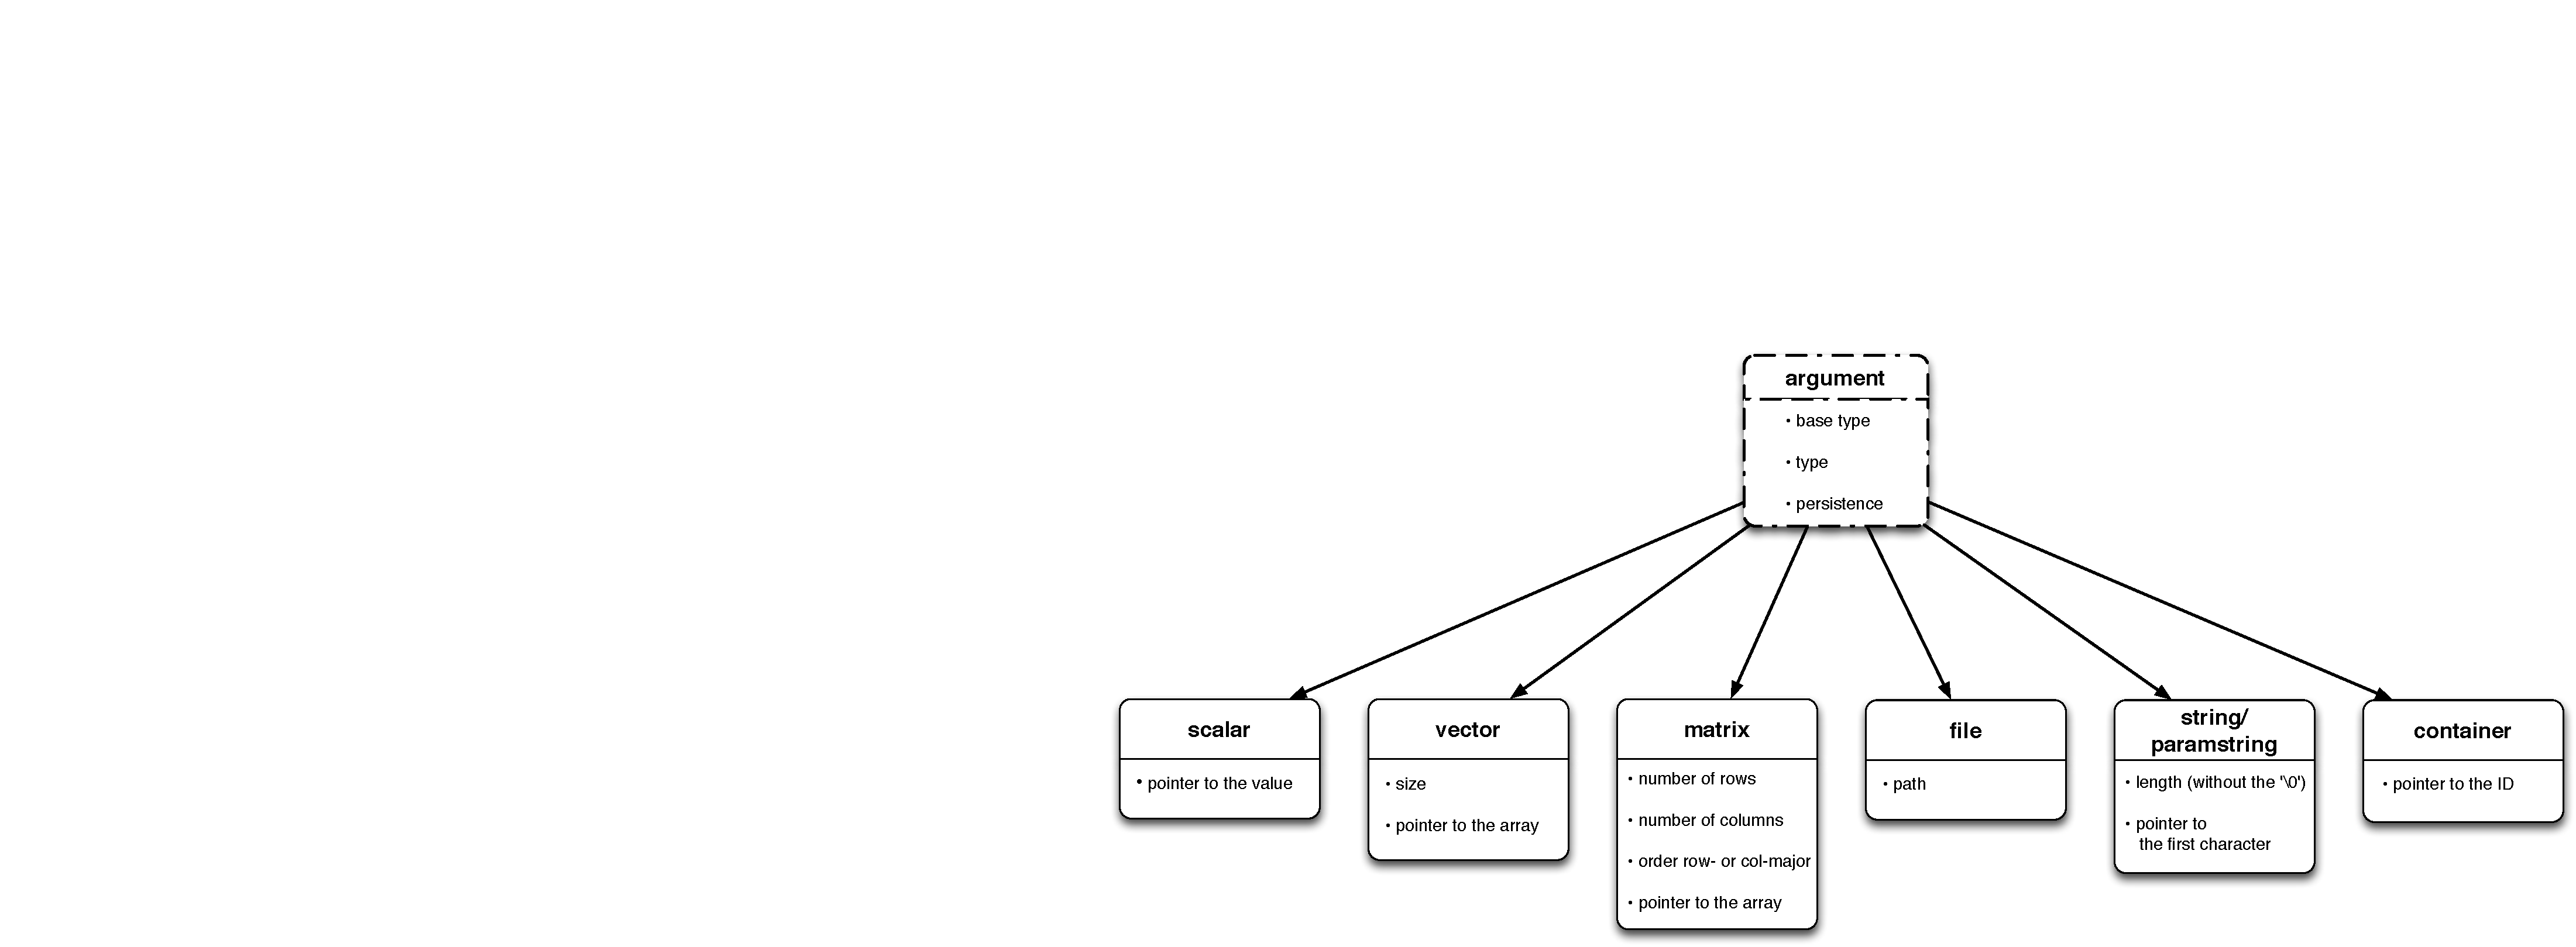
\includegraphics[scale=.5]{fig/data.eps}
  \caption{Argument/Data structure description}
  \label{fig:data}
 \end{center}
\end{figure}



\section{Manipulating DIET structures}
\label{sec:manip}

The user will notice that the API to the DIET data structures consists of
modifier and accessor functions only: no allocation function is required, since
\texttt{diet\_profile\_alloc} (see Section \ref{sec:pbdesc}) allocates all
necessary memory for all argument \textbf{descriptions}. This avoids the
temptation for the user to allocate the memory for these data structures twice
(which would lead to DIET errors while reading profile arguments). Please see
the example in Section \ref{sec:pbex} for a typical use.
\\

Moreover, the user should know that arguments of the \texttt{\_set} functions
that are passed by pointers are \textbf{not} copied, in order to save memory.
This is true for the \emph{value} arguments, but also for the \emph{path} in
\texttt{diet\_file\_set}. Thus, the user keeps ownership of the memory zones
pointed at by these pointers, and he/she must be very careful not to alter it
during a call to DIET.

\subsection{Set functions}
\label{sec:setfun}
{\footnotesize
\begin{verbatim}
/**
 * On the server side, these functions should not be used on arguments, but only
 * on convertors.
 * If mode                             is DIET_PERSISTENCE_MODE_COUNT,
 * if base_type                        is DIET_BASE_TYPE_COUNT,
 * if order                            is DIET_MATRIX_ORDER_COUNT,
 * if size, nb_rows, nb_cols or length is 0,
 * if path                             is NULL,
 * then the correspunding field is not modified.
 */

int
diet_scalar_set(diet_arg_t* arg, void* value, diet_persistence_mode_t mode,
                diet_base_type_t base_type);
int
diet_vector_set(diet_arg_t* arg, void* value, diet_persistence_mode_t mode,
                diet_base_type_t base_type, size_t size);

/* Matrices can be stored by rows or by columns */
typedef enum {
  DIET_COL_MAJOR = 0,
  DIET_ROW_MAJOR,
  DIET_MATRIX_ORDER_COUNT
} diet_matrix_order_t;

int
diet_matrix_set(diet_arg_t* arg, void* value, diet_persistence_mode_t mode,
                diet_base_type_t base_type,
                size_t nb_rows, size_t nb_cols, diet_matrix_order_t order);
int
diet_string_set(diet_arg_t* arg, char* value, diet_persistence_mode_t mode,
                size_t length);
/* Computes the file size
   ! Warning ! The path is not duplicated !!! */
int
diet_file_set(diet_arg_t* arg, diet_persistence_mode_t mode, char* path);
\end{verbatim}
}

\subsection{Access functions}
\label{sec:accessfun}
{\footnotesize
\begin{verbatim}
/**
 * A NULL pointer is not an error (except for arg): it is simply IGNORED.
 * For instance,
 *   diet_scalar_get(arg, &value, NULL),
 * will only set the value to the value field of the (*arg) structure.
 * 
 * NB: these are macros that let the user not worry about casting its (int **)
 * or (double **) etc. into (void **).
 */

/**
 * Type: int diet_scalar_get((diet_arg_t *), (void *),
 *                           (diet_persistence_mode_t *))
 */
#define diet_scalar_get(arg, value, mode) \
        _scalar_get(arg, (void *)value, mode)
/**
 * Type: int diet_vector_get((diet_arg_t *), (void **),
 *                           (diet_persistence_mode_t *), (size_t *))
 */
#define diet_vector_get(arg, value, mode, size) \
        _vector_get(arg, (void **)value, mode, size)
/**
 * Type: int diet_matrix_get((diet_arg_t *), (void **),
 *                           (diet_persistence_mode_t *),
 *                           (size_t *), (size_t *), (diet_matrix_order_t *))
 */
#define diet_matrix_get(arg, value, mode, nb_rows, nb_cols, order) \
        _matrix_get(arg, (void **)value, mode, nb_rows, nb_cols, order)
/**
 * Type: int diet_string_get((diet_arg_t *), (char **),
 *                           (diet_persistence_mode_t *), (size_t *))
 */
#define diet_string_get(arg, value, mode, length) \
        _string_get(arg, (char **)value, mode, length)
/**
 * Type: int diet_file_get((diet_arg_t *),
 *                         (diet_persistence_mode_t *), (size_t *), (char **))
 */
#define diet_file_get(arg, mode, size, path) \
        _file_get(arg, mode, size, (char **)path)
\end{verbatim}
}


\subsection{Free functions}
\label{sec:freefun}

The amount of data  pointed at by value fields should be freed through a DIET
API function:
{\footnotesize
\begin{verbatim}
/****************************************************************************/
/* Free the amount of data pointed at by the value field of an argument.    */
/* This should be used ONLY for VOLATILE data,                              */
/*    - on the server for IN arguments that will no longer be used          */
/*    - on the client for OUT arguments, after the problem has been solved, */
/*      when they will no longer be used.                                   */
/* NB: for files, this function removes the file and frees the path (since  */
/*     it has been dynamically allocated by DIET in both cases)             */
/****************************************************************************/

int
diet_free_data(diet_arg_t* arg);
\end{verbatim}
}


\section{Problem description}
\label{sec:pbdesc}

For DIET to match the client problem with a service, servers and clients must
``speak the same language'', \emph{ie} they must use the same problem
description. A unified way to describe problems is to use a name and define its
profile with the type \texttt{diet\_profile\_t}:
{\footnotesize
\begin{verbatim}
typedef struct {
  int         last_in, last_inout, last_out;
  diet_arg_t *parameters;
} diet_profile_t;
\end{verbatim}
}

%
% FIXME:
% as soon as persistency is integrated, this should become the table Eddy
% prepared to explain the transfer policy, depending on the modes.
%

The field \emph{parameters} consists of a \texttt{diet\_arg\_t} array of size
$last\_out + 1$. An argument can be
\begin{description}
\item{IN:}    The data are sent to the server. The memory is allocated
  by the user.
\item{INOUT:} The data are allocated by the user as for the IN
  arguments, then sent to the server and brought back into the same memory zone
  after the computation has completed, without any copy. Thus freeing this
  memory while the computation is performed on the server would result in a
  segmentation fault when the data are brought back onto the client.
\item{OUT:} The data are created on the server and brought back into a
  newly allocated zone on the client. After the call has returned, the user can
  find its result in the zone pointed at by the \emph{value} field. Of course,
  DIET cannot guess how long the user needs these data for, so it lets him/her
  free the memory allocated with \texttt{diet\_free\_data}.
\end{description}

This behaviour will be modified soon with the introduction of the persistence
modes that will let the user leave some data on the servers for later
computations.

The fields \emph{last\_in}, \emph{last\_inout} and \emph{last\_out} of the
\texttt{diet\_profile\_t} structure respectively point at the indexes in the
\emph{parameters} array of the last IN, INOUT and OUT arguments.

Functions to create and destroy such profiles are defined with the prototypes
below:
{\footnotesize
\begin{verbatim}
diet_profile_t *diet_profile_alloc(int last_in, int last_inout, int last_out);
int diet_profile_free(diet_profile_t *profile);
\end{verbatim}
}



\section{Example}
\label{sec:pbex}

Let us consider the product of a scalar by a matrix: the matrix must be
multiplied in-place, and the computation time must be returned.  Typically, this
problem has one IN argument (the scalar factor), one INOUT argument (the matrix)
and one OUT argument (the computation time), so its profile will be built as
follows:
\begin{center}
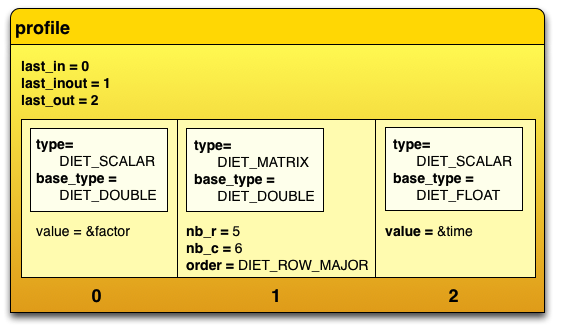
\includegraphics[scale=.35]{fig/smprod.eps}
\end{center}

Here are the lines of C code to generate such a profile:
{\footnotesize
\begin{verbatim}
  double  factor;
  double *matrix;
  float  *time;
  // Init matrix at least, factor and time too would be better ...
  // ...
  diet_profile_t profile = diet_profile_alloc(0, 1, 2); // last_in, last_inout, last_out
  diet_scalar_set(diet_parameter(profile,0), &factor, 0, DIET_DOUBLE);
  diet_matrix_set(diet_parameter(profile,1), matrix,  0, DIET_DOUBLE, 5, 6, DIET_ROW_MAJOR);
  diet_scalar_set(diet_parameter(profile,2), NULL,    0, DIET_FLOAT);
\end{verbatim}
}

\noindent

\textbf{NB1:} If there is no IN argument, \emph{last\_in} must be set to -1, if
there is no INOUT argument is needed, \emph{last\_inout} must be equal to
\emph{last\_in}, and if there is no OUT argument, \emph{last\_out} must be equal
to \emph{last\_inout}.\\
\textbf{NB2:} The \emph{value} argument for \texttt{\_set} functions
(\ref{sec:setfun}) is ignored for OUT arguments, since DIET allocates the
necessary memory space when the corresponding data are transfered from the
server, so set it to NULL.


